% ===================================
% FIGURA 1.4 - VERSIONE ALTERNATIVA
% Con posizionamento assoluto per evitare problemi
% ===================================
\documentclass[tikz,border=10pt]{standalone}
\usepackage[T1]{fontenc}
\usepackage{tikz}
\usetikzlibrary{arrows.meta, shadows}

\begin{document}
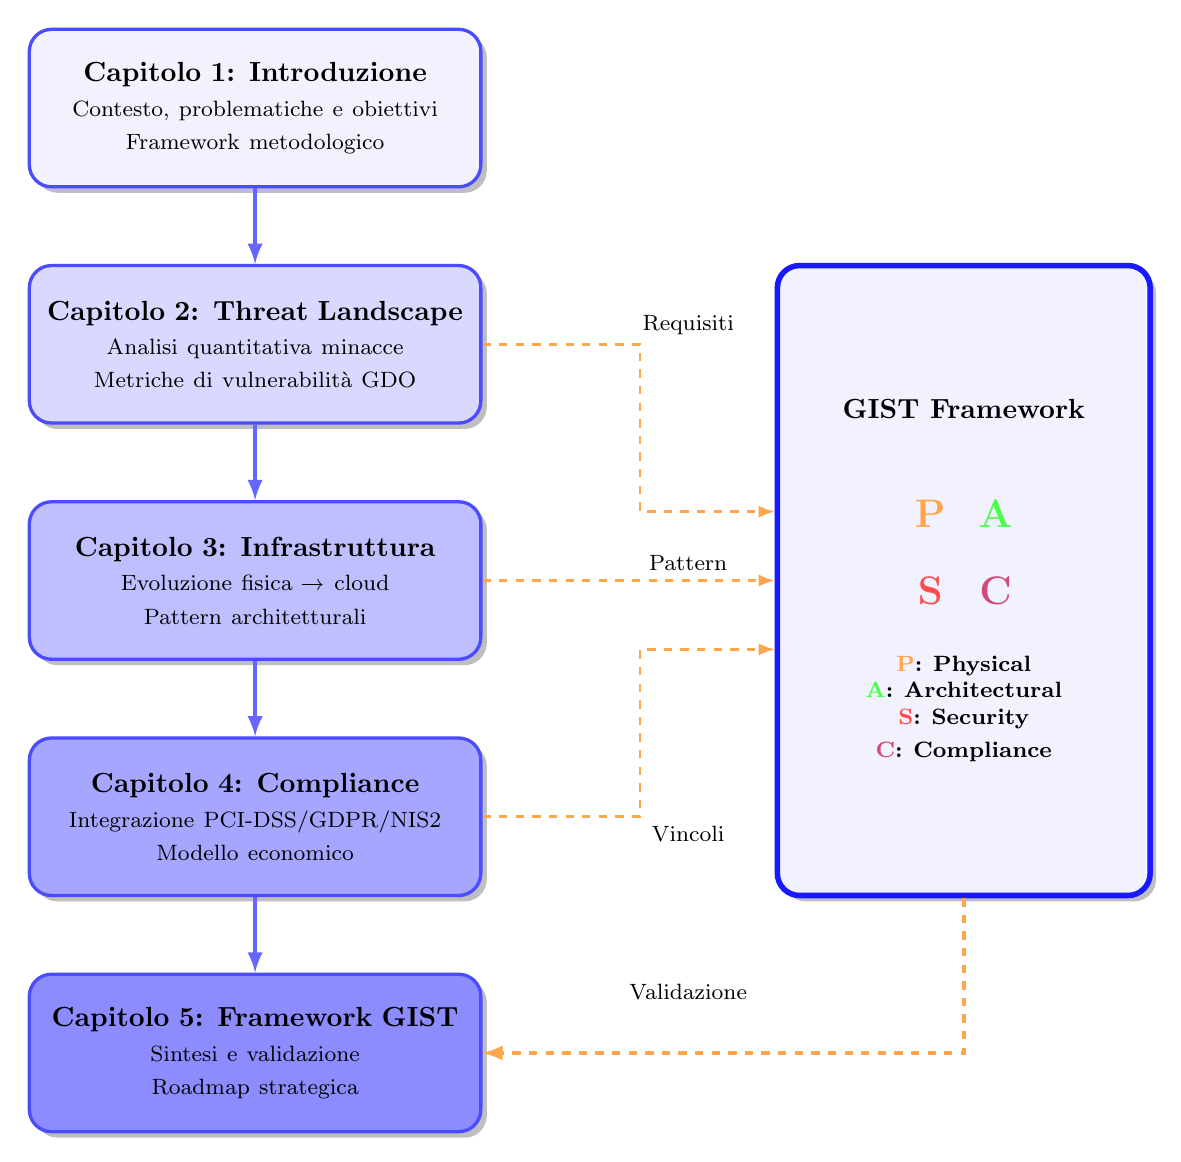
\begin{tikzpicture}
    % Definizione stili
    \tikzset{
        chapter/.style={
            rectangle, 
            draw=blue!70, 
            fill=blue!#1, 
            text width=5.5cm, 
            text centered, 
            rounded corners=8pt, 
            minimum height=2cm, 
            font=\normalsize, 
            line width=1.2pt, 
            drop shadow
        },
        arrow/.style={->, >=latex, line width=1.5pt, draw=blue!60},
        feedback/.style={->, >=latex, line width=1pt, draw=orange!70, dashed}
    }

    % Posizionamento assoluto dei capitoli
    \node[chapter=5] at (0,0) (cap1) {
        \textbf{Capitolo 1: Introduzione}\\[3pt]
        \footnotesize Contesto, problematiche e obiettivi\\
        Framework metodologico
    };
    
    \node[chapter=15] at (0,-3) (cap2) {
        \textbf{Capitolo 2: Threat Landscape}\\[3pt]
        \footnotesize Analisi quantitativa minacce\\
        Metriche di vulnerabilità GDO
    };
    
    \node[chapter=25] at (0,-6) (cap3) {
        \textbf{Capitolo 3: Infrastruttura}\\[3pt]
        \footnotesize Evoluzione fisica → cloud\\
        Pattern architetturali
    };
    
    \node[chapter=35] at (0,-9) (cap4) {
        \textbf{Capitolo 4: Compliance}\\[3pt]
        \footnotesize Integrazione PCI-DSS/GDPR/NIS2\\
        Modello economico
    };
    
    \node[chapter=45] at (0,-12) (cap5) {
        \textbf{Capitolo 5: Framework GIST}\\[3pt]
        \footnotesize Sintesi e validazione\\
        Roadmap strategica
    };

    % Framework GIST
    \node[
        rectangle, 
        draw=blue!90, 
        fill=blue!5, 
        text width=4.5cm, 
        text centered, 
        rounded corners=8pt, 
        minimum height=8cm,
        font=\normalsize\bfseries, 
        line width=2pt, 
        drop shadow
    ] at (9,-6) (gist) {
        \textbf{GIST Framework}\\[1cm]
        \begin{tabular}{cc}
            \textcolor{orange!70}{\Large\textbf{P}} & \textcolor{green!70}{\Large\textbf{A}}\\[0.5cm]
            \textcolor{red!70}{\Large\textbf{S}} & \textcolor{purple!70}{\Large\textbf{C}}
        \end{tabular}\\[0.5cm]
        \footnotesize
        \textcolor{orange!70}{P}: Physical\\
        \textcolor{green!70}{A}: Architectural\\
        \textcolor{red!70}{S}: Security\\
        \textcolor{purple!70}{C}: Compliance
    };

    % Frecce tra capitoli
    \draw[arrow] (cap1.south) -- (cap2.north);
    \draw[arrow] (cap2.south) -- (cap3.north);
    \draw[arrow] (cap3.south) -- (cap4.north);
    \draw[arrow] (cap4.south) -- (cap5.north);

    % Frecce di feedback
    \draw[feedback] (cap2.east) -- ++(2,0) |- (gist.160);
    \draw[feedback] (cap3.east) -- (gist.west);
    \draw[feedback] (cap4.east) -- ++(2,0) |- (gist.200);
    \draw[feedback, line width=1.5pt] (gist.south) |- (cap5.east);
    
    % Etichette
    \node[font=\footnotesize, above] at (5.5,-3) {Requisiti};
    \node[font=\footnotesize, above] at (5.5,-6) {Pattern};
    \node[font=\footnotesize, below] at (5.5,-9) {Vincoli};
    \node[font=\footnotesize, below] at (5.5,-11) {Validazione};

\end{tikzpicture}
\end{document}